\section{Theoretische Grundlagen}

\subsection{Tunneleffekt}

Der Tunneleffekt ist ein quantenmechanischer Effekt, der Teilchen erlaubt, endlich hohe Potentialbarrieren zu überwinden. In diesem Potentialbereich nimmt die Amplitude der Wellenfunktion exponentiell ab. Hinter diesem Bereich ist sie also viel kleiner als vor dem Bereich. Das Quadrat der Amplitude beschreibt die Wahrscheinlichkeitsdichte und somit kann man den Amplitudenabfall als Tunnelwahrscheinlichkeit interpretieren.
Beim Rastertunnelmikroskop wird dieser Effekt ausgenutzt um nach Anlegen einer Potentialdifferenz zwischen Spitze und Probe den Tunnelstrom zu messen und somit die Distanz zwischen diesen beiden Komponenten zu messen (siehe hierzu den Abschnitt \emph{Das Rastertunnelmikroskop}).

\subsection{Halbleiter}


Halbleiter sind Materialien, deren elektrische Leitfähigkeit mit ihrer Temperatur steigt. Bei tiefen Temperaturen ist die Leitfähigkeit hingegen gering. Man unterscheidet zwischen Elementhalbleiter, die aus einzelnen Elementen bestehen, und Verbindungshalbleiter, die aus chemischen Bindungen oder Legierungen bestehen. Bei einer Temperatur von $T=0 \ K$ ist das Valenzband des Halbleiters komplett besetzt und das Leitungsband leer (Alle Elektronen haben eine kleinere Energie als die Fermienergie). Der Halbleiter hat also die Eigenschaften eines Isolators, jedoch ist die Lücke zwischen Valenz- und Leitungsband kleiner, kann also durch verschiedene Methoden überwunden werden. Zum Beispiel kann die Temperatur $T$ des Materials erhöht werden. Eine Temperaturerhöhung würde den Elektronen Energie zufügen, mit welcher sie die Lücke überwinden könnten. Daher die Abhängigkeit der Leitfähigkeit von der Temperatur: Steigt diese, so steigt die Anzahl der Elektronen, die in das Leitungsband übergehen können und somit die Leitfähigkeit. Jedes Elektron, das in das Leitungsband gelangt hinterlässt ein "`Loch"' (im unteren Bild als Defektelektron bezeichnet), welches als fehlende negative Ladung wie ein positiver Ladungsträger erscheint. Die Elektronendichte im Leitungsband ist dann das Produkt aus Zustandsdichte und Fermi-Verteilung und Zahl der Spinorientierungen (also 2). Eine andere Möglichkeit ist die Dotierung, d.h. das Einbringen von Fremdatomen in sehr kleinen Mengen, die als Störstellen agieren und somit die Materialeigenschaften wie die Leitfähigkeit ändern können.

\begin{figure}[H]
	\centering 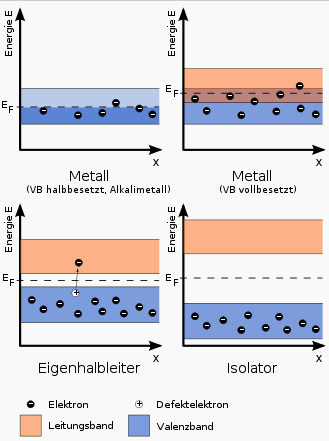
\includegraphics[width=0.6\textwidth]{Bilder/Halbleiter.png}
	\caption{Vergleich zwischen Halbleiter und anderen Stoffen (\emph{wikipedia.de})}
\end{figure}

\subsection{Piezoelektrischer Effekt}

Durch Anlegen einer Spannung an ein sogenanntes piezoelektrisches Material, entstehen innerhalb von diesem Dipolmomente, da die Ladungen von der Spannung "`auseinandergezogen"' werden. Diese Dipolmomente, da sie so zahlreich sind, ändern die gesamte Form des Materials. Man kann also das Material anhand von Spannungen beliebig verformen. Dieser Effekt hat den Vorteil, dass man diese Verformung sehr genau machen kann. In unserem Versuch nutzen wir den Effekt aus, um die Spitze sehr genau einzustellen bzw. nachzuführen. Die Genauigkeit beträgt $150 \mathring A/V$, d.h. der Computer kann die Spitze mit einer Genauigkeit von weniger als $1 \mathring A$ einstellen.

\subsection{Struktur von Gold}

Da Gold ein reines Metall ist, sind die Elektronen zwischen den Atomen komplett delokalisiert. Die Elektronen sind frei beweglich und gehören zu keinem Kern, sind also nicht in Orbitalen. Die Elektronendichte zeigt also kaum Variation. Bei der Messung können wir somit nicht erwarten, atomare Auflösung zu erhalten.

\subsection{Struktur von Graphit}

\begin{figure}[H]
	\centering 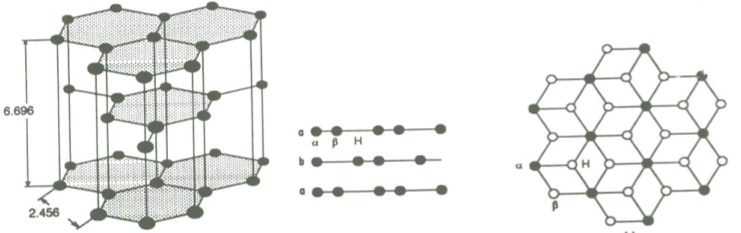
\includegraphics[width=\textwidth]{Bilder/Graphit.png}
	\caption{Kristallstruktur von Graphit (Längen in $\mathring{A})$}
\end{figure}

Graphit besteht aus übereinanderliegenden Schichten von Kohlenstoffatomen, welche in Sechs\-ecken angeordnet sind. Die Atome in einer Schicht sind durch kovalente, lokalisierte $\sigma$-Bindungen und durch nichtlokalisierte $\pi$-Bindungen verbunden. Die Elektronen der $\pi$-Bindung bewegen sich frei in den Schichten. Dies erklärt die Halbmetalleigenschaft des Graphits: Die delokalisierten Elektronen können Strom nur parallel zu den Schichten leiten, aber nicht senkrecht. Die Schichten halten durch Van-der-Waals-Kräfte zusammen. Man unterscheidet beim Graphit zwischen den $\alpha$- und den $\beta$-Kohlenstoffatomen (siehe hierzu obere Abbildung). Die $\alpha$-Atome, sind die Atome unter denen in jeder Schicht nochmal ein $\alpha$-Atom liegt. Die $\beta$-Atome hingegen liegen nur in jeder zweiter Schicht, d.h. in der Schicht darunter ist ein Loch und darunter wieder ein $\beta$-Atom. Da die $\alpha$-Atome mit den $\alpha$-Atomen der unteren Schichten koppeln, ist die Energie deren Elektronen erniedrigt. Die $\beta$-Atome sind mit dem Rastertunnelmikroskop also besser sichtbar. Man sieht also eher ein dreieckiges Gitter aus $\beta$-Atomen als eine sechseckige Wabenstruktur.

\subsection{Struktur von $MoS_2$}

\begin{figure}[H]
	\centering 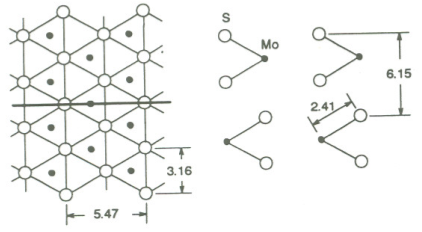
\includegraphics[width=0.8\textwidth]{Bilder/MoS2.png}
	\caption{Kristallstruktur und Cross-section von $MoS_2$ (Längen in $\mathring{A})$}
\end{figure}

Molybdändisulfid ist ein Halbleiter mit einer Energiebandlücke von 0.75 eV. Es besteht aus Schichten, in denen alle Valenzelektronen Bindungen eingehen. Die Schichten sind wie beim Graphit durch Van-der-Waals-Kräfte verbunden. Wie man auf dem oberen Bild sieht, besteht das $MoS_2$ aus Schichten von Molybdän-Atomen, die sich wie ein Diamantgitter anordnen. Die Molybdän-Schicht befindet sich zwischen zwei Schwefelschichten, die auch ein Diamantgitter bilden, jedoch verschoben zu dem Molybdän-Gitter. Im Idealfall kann man beim Rastertunnelmikroskop zwischen den S- und den Mo-Atomen unterscheiden.

\subsection{Funktionsprinzip des Rastertunnelmikroskops}

Eine im Idealfall atomar scharfe metallische Spitze wird an eine Probenoberfläche auf einen Abstand von ca. $10 \mathring A$ herangeführt . Legt man eine Potentialdifferenz U zwischen Spitze und Probe an, so fließt zwischen Probe und Spitze ein Tunnelstrom I. Für die Stromstärke gilt näherungsweise folgende Abhängigkeit:

$$ I \sim U\exp\left(-\sqrt{\frac{2\pi\Phi}{\hbar}}\cdot d\right) $$

$\Phi$ ist die effektive lokale Höhe der Barriere, die durchtunnelt wird, und $d$ die Distanz der Probe zu Spitze. Man sieht also dass die Stromstärke exponentiell von dieser abhängt. Der Strom I liegt typischerweise im Nano-Ampere-Bereich.

\begin{figure}[H]
\begin{minipage}{0.5\textwidth}
	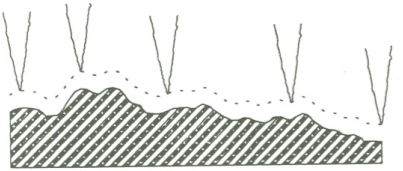
\includegraphics[width=0.9\textwidth]{Bilder/CCM.png}
	\centering \caption{Nachführen der Spitze}
\end{minipage}
\begin{minipage}{0.5\textwidth}
Durch die Messung des Tunnelstromes kann man also den relativen Abstand der Spitze zur Probe feststellen (Je stärker der Tunnelstrom, desto näher ist die Spitze an der Probe und umgekehrt). Misst  der eingebaute Regelkreis eine Abnahme der Stromstärke, so wird die Spitze näher an die Probe herangefahren, bis wieder der eingestel\-lte Strom fließt. Dasselbe gilt bei Zunahme des Stroms, die Spitze wird wegbewegt. Das Raster-
\end{minipage}
\end{figure}
tunnelmikroskop zeichnet somit die Topographie der Oberfläche der Probe, indem es die Bewegung der Spitze registriert. Die Spitze wird anhand eines Piezo-Kristalls nachgeführt um eine bestmögliche Genauigkeit zu erreichen, und um die Bewegung der Spitze anhand der angelegten Spannung an das Kristall zu registrieren.

Die hier erklärte Messungsweise wird \emph{Constant Current Mode} genannt, da die Stromstärke konstant bleibt. Eine weitere Methode ist die \emph{Constant Height Mode}, bei der die Spitze immer die gleiche Höhe behält und durch die Stärke des Tunnelstroms die Distanz von der Spitze zur Probe misst. Letztere Methode wird aber im Versuch nicht benutzt.

\begin{figure}[H]
\begin{minipage}{0.5\textwidth}
Nicht nur die Stromstärke sondern auch die Auflösung des Rastertunnelmikroskops hängt von der Distanz der Spitze zur Probe ab. Außerdem hängt sie von der Breite der Spitze ab. Sei R die räumliche Ausdehnung der Spitze, so gilt für das laterale Auflösungsvermögen L des Rastertunnelmikroskops folgende Abhängigkeit:

$$ L \sim \sqrt{R+d} $$

\end{minipage}
\begin{minipage}{0.5\textwidth}
	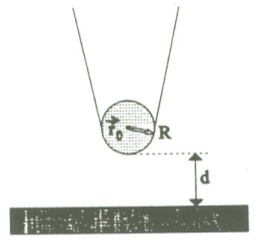
\includegraphics[width=0.6\textwidth]{Bilder/auflsg.png}
	\centering \caption{Zur lateralen Auflösung des RTM}
\end{minipage}
\end{figure}

Um genaue Messungen machen zu können ist es außerdem sehr wichtig, dass die externen Störungen minimiert werden. Wichtige Störparameter sind vor allem Temperaturschwankungen (wegen der temperaturabhängigen Ausdehnung von der Metallspitze) und Vibrationen. Temperaturschwankungen sind am leichtesten durch Abdichtung des Raumes zu verhindern und im Raum selber keine Heiz- bzw. Kühlkorper zu haben. Vibrationen, wie Trittschall und Gebäudeschwingungen können mit speziellen Vibrationsisolierungen minimiert werden. 

\clearpage
